\documentclass[a4paper,utf8]{article}
\usepackage{graphicx}
\usepackage[heading,fancyhdr]{ctex}
\usepackage{amsmath,amssymb,geometry,ulem}
\usepackage{array,tabularx,tabulary,mhchem,xspace}
\usepackage{floatrow,subfig,multirow,bigstrut}
\usepackage{siunitx,booktabs,longtable,nameref}
\lineskiplimit=1pt
\lineskip=3pt
\geometry{
    top=25.4mm, 
    left=25mm, 
    right=25mm, 
    bottom=25mm,
    headsep=5.9mm,
}
\ctexset{
    chapter = {
        name = {实验,},
        beforeskip = {-23pt}
    }
}
\newcommand{\fgref}[1]{图~\ref{#1}\xspace}
\newcommand{\seqref}[1]{式~(\ref{#1})}
\newcommand{\expinfo}[6][无]{
    {\zihao{-3}\bfseries\songti
    实验名称:\uline{\hfill\mbox{#2}\hfill} \\[2.9mm]
    学\quad 号:\uline{\makebox[25mm]{#3}}\hfill
    姓\quad 名:\uline{\makebox[25mm]{#4}}\hfill
    班\quad 级:\uline{\makebox[25mm]{#5}} \\[2.9mm]
    合作者:\uline{\makebox[25mm]{#1}} \hfill
    桌\quad 号:\uline{\makebox[25mm]{}}\hfill\makebox[25mm+4em]{}\\[2.9mm]
    指导教师:\uline{\makebox[30mm]{#6}}\hfill\mbox{} \\[2.9mm]
    实验日期:\uline{\makebox[30mm]{}}\hfill\mbox{} \\[58.7mm]
    }
}%\expinfo[合作者]{实验名称}{学号}{姓名}{班级}{指导教师}
\newcommand{\pointingbox}{
    {\zihao{4}\bfseries\songti%
    实验考核\\[3mm]
    \extrarowheight=3mm
    \begin{tabularx}{150mm}{|X|X|X|X|X|}\hline
        \hfil 项目 \hfil  & \hfil 实验预习 \hfil & \hfil 实验过程 \hfil & \hfil 分析与讨论 \hfil & \hfil 总评 \hfil \\[3mm] \hline
        \hfil 评价 \hfil &  &  &  &  \\[3mm] \hline
    \end{tabularx}
    }
}
\newcommand{\derivative}[2]{\frac{\mathrm{d} #1}{\mathrm{d} #2}}
\newcommand{\thinking}[2]{\textbf{#1}\\
答:\begin{minipage}[t]{0.85\textwidth}
    #2
\end{minipage}}

\pagestyle{fancy}
\fancyhf{}
%\fancyhead[C]{材料科学基础实验}
%\fancyfoot[C]{\thepage}
\fancyhead[EC]{\leftmark} \fancyhead[OC]{\rightmark}
\fancyhead[EL,OR]{\thepage}
\fancypagestyle{plain}{\renewcommand{\headrulewidth}{0pt}\fancyhf{}}

\newcounter{Rownumber}
\newcommand*{\Rown}{\stepcounter{Rownumber}\theRownumber}
\newcounter{sample}
\newcommand*{\Sam}{\stepcounter{sample}\thesample}
\newcounter{Fignumber}
\newcommand*{\Fign}{\stepcounter{Fignumber}\theFignumber}

\newcommand*{\resetRown}{\setcounter{Rownumber}{0}}
\newcommand{\qrange}[3]{\qtyrange[range-phrase = \text{$\sim$},range-units =single]{#1}{#2}{#3}}
\floatsetup[table]{capposition=top}
\newcolumntype{C}{>{\hfil}X<{\hfil}}
\renewcommand{\Nameref}[1]{\textbf{\ref{#1}~\nameref{#1}}}
\newcommand{\TTR}[0]{\watt\per\m\per\K}
\begin{document}
\begin{center}
    {\mbox{}\\[7em]\zihao{2}\bfseries\songti%
    材料科学基础实验预习报告}\\[34mm]
    \expinfo{碳钢淬火、回火后的组织观察与硬度分析}{22301077}{张蕴东}{22高分子}{杨玉华}
    \pointingbox
\end{center}\newpage
\section{实验目的}
    \begin{enumerate}
        \item 了解碳钢的淬火、回火过程。
        \item 观察和研究碳钢经不同淬火、回火处理后显微组织的特点,分析冷却条件、淬火温度及回火条件对其组织形态与硬度的影响,并了解淬火、回火的应用领域。
    \end{enumerate}
\section{实验原理}%简单描述,含必要的公式和附图;
    热处理包括四个因素:加热速度、最高温度、加热时间(通常将工件升温和保温所需时间算在一起,统称为加热时间)和冷却速度。根据热处理工艺的使用和进行方式不同,热处理一般可分为下列四种类型:退火、正火、淬火、回火。\par
    \subsection{淬火}
        将钢奥氏体化后以大于临界冷却速度的速度进行冷却,获得马氏体或下贝氏体组织的热处理工艺,称为淬火。钢淬火的主要目的是为了获得马氏体,提高它的硬度和强度。
        \subsubsection{淬火温度的选择}
            根据钢的相变点选择淬火加热温度,主要以获得细小均匀的奥氏体为主,一般原则是:亚共析钢为$A_{3}+(30{\sim}50)~\unit{\degreeCelsius}$($A_3$ 线是钢 $\alpha$ 固溶体转变为 $\gamma$ 固溶体之临界温度),共析钢和过共析钢$A_{1}+(30{\sim}50)~\unit{\degreeCelsius}$($A_1$ 为共析转变温度),如\fgref{fig:1} 所示。
            \begin{figure}[!ht]
                \caption{淬火的加热温度范围\label{fig:1}}
                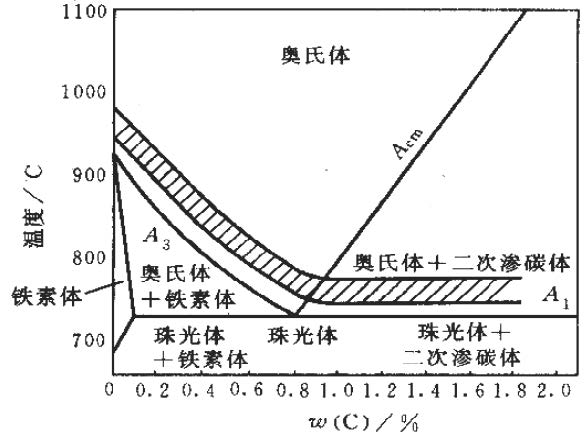
\includegraphics[width=60mm]{fig1.jpg}
            \end{figure}
        \subsubsection{保温时间}
            保温的目的是使钢件热透,使奥氏体充分转变为均匀化。保温时间的长短主要根据钢的成分、加热介质和零件尺寸决定,计算公式为
            \begin{equation}
                \tau=\alpha KD
            \end{equation}
            式中,$\alpha$ 为加热系数;$K$ 为装炉系数;$D$ 为有效尺寸。
        \subsubsection{淬火冷却介质}
            钢在加热获得奥氏体后要选用适当的冷却介质进行冷却,获得马氏体组织。
        \subsubsection{淬火后的组织}
            亚共析钢淬火后得到马氏体组织,马氏体组织为板条状或针状,低碳钢(碳含量小于 0.25\% 的非合金钢)淬火后的组织在光学显微镜下,其形态为一束束接近相互平行的细条状马氏体群。\par
            中碳钢(碳含量界于 $0.25\%-0.6\%$ 之间的非合金钢)经正常淬火后将得到细针状马氏体和板条状马氏体的混合组织。高碳钢(碳含量大于 $0.6\%$ 的非合金钢)如共析钢和过共析钢在等温淬火后可得到贝氏体组织。上贝氏体是由成束平行排列的条状铁素体和条间断分布的渗碳体组成的片层状组织;当转变量不多时,在光学显微镜下可看到成束的铁素体由奥氏体晶界向内伸展,具有羽毛特征。下贝氏体是在片状铁素体内部沉淀有碳化物的组织;由于易受浸蚀,所以在显微镜下呈黑色针状特征。\par
            共析钢和过共析钢在淬火后亦得到马氏体组织,如 T8 钢淬火后除得到针状马氏体外,还有较多的残余奥氏体。高碳马氏体呈片状,片间互成一定角度。
    \subsection{回火}
        回火是将经过淬火的试样加热到临界点 $A_1$ 以下的适当温度,保持一定时间后,采用适当的冷却方式进行冷却,以获得所需的组织和性能的热处理工艺。根据回火温度的不同,回火可分为低温回
        火($150 \sim 250~\unit{\degreeCelsius}$)、中温回火($350 \sim 500~\unit{\degreeCelsius}$)和高温回火($500 \sim 650~\unit{\degreeCelsius}$)三种。
            \subsubsection{回火马氏体}
                经低温回火后,从淬火马氏体内脱溶沉淀析出高度弥散的与母相保持着共格联系的碳化物质点的组织。
            \subsubsection{回火屈氏体}
                经中温回火后,在铁素体基体上弥散分布着微小粒状的渗碳体组织。
            \subsubsection{回火索氏体}
                经高温回火后,由颗粒状渗碳体和多边形的铁素体组成的组织。45 钢经淬火+高温回火后的组织如\par
                回火所得到的回火索氏体和回火屈氏体与由过冷奥氏体直接分解出来的索氏体和屈氏体在显微组织上是不同的,前者中的渗碳体呈粒状而后者则为片状。
\section{实验仪器}%规格及参数
箱式电阻加热炉,洛氏硬度计,砂纸,抛光机,金相显微镜。热处理试样:45 钢。冷却介质水和油及淬火水桶,长柄铁钳等。
\section{实验过程}%简述主要过程和实验内容
    \begin{enumerate}
        \item 每4人一组,领取45钢(4个),每组共同完成一套实验(对应下表中相应的热处理工艺方法)。
        \begin{table}[!ht]\centering
            \caption{试样的热处理工艺}
            \newcounter{sample} \newcommand{\Sam}{\stepcounter{sample}\thesample}
            \begin{tabular}{c c c c c}\hline
                试样号码 & 钢号 & 热处理工艺 & 浸蚀剂 & 建议放大倍数 \\ \hline
                \Sam & 45 & 淬火,油冷 & 4\% 硝酸酒精 & 200 $\sim$ 500 \\ \hline
                \Sam & 45 & 淬火,水冷 & 4\% 硝酸酒精 & 200 $\sim$ 500 \\ \hline
                \Sam & 45 & 淬火+中温回火 & 4\% 硝酸酒精 & 200 $\sim$ 500 \\ \hline
                \Sam & 45 & 淬火+高温回火 & 4\% 硝酸酒精 & 200 $\sim$ 500 \\ \hline
            \end{tabular}
        \end{table}
        \item 制定热处理工艺参数,加热温度和淬火冷却方式按照表中给定的实施,淬火加热保温时间根据给定试样的尺寸,依据公式计算求得(20-30 分钟),回火保温时间均采用 1 小时且均采用空冷方式。
        \begin{enumerate}
            \item 45 钢淬火工艺:加热温度为 $860 \pm \SI{10}{\degreeCelsius}$,根据试样有效尺寸计算保温时间,保温后用长柄铁钳夹出放入\textbf{淬火油}中冷却。
            \item 45 钢淬火工艺:加热温度为 $860 \pm \SI{10}{\degreeCelsius}$,根据试样有效尺寸计算保温时间,保温后用长柄铁钳夹出放入\textbf{水}中进行冷却。
            \item 45 钢淬水+中温回火工艺:加热温度为 $860 \pm \SI{10}{\degreeCelsius}$,根据试样有效尺寸计算保温时间,保温后出炉进行水淬。随后放入炉中加热至 \SI{400}{\degreeCelsius},保温 1 个小时后出炉空冷。
            \item 45 钢淬水+高温回火工艺:加热温度为 $860 \pm \SI{10}{\degreeCelsius}$,根据试样有效尺寸计算保温时间,保温后出炉进行水淬。随后放入炉中加热至 \SI{600}{\degreeCelsius},保温 1 个小时后出炉空冷。
        \end{enumerate}
        \item 利用硬度计对\textbf{所有热处理后的试样进行硬度测试},每个试样至少三个试验点,再取一个平均值。\textbf{进行回火的试样需进行两次硬度测试,即淬火后回火前、回火后两次},测试结果记录于下表中。(硬度测试须在金相磨制观察前完成)
        \item 根据拟定的热处理工艺对试样进行相应的热处理,然后利用金相砂纸对热处理后的试样进行\textbf{磨制、抛光},并用 $4\%$ 的硝酸酒精进行腐蚀制得金相试样。\textbf{利用金相显微镜对其进行显微组织观察,分析热处理工艺对其组织的影响。}
        \item 实验结束后,汇总各小组实验数据,根据实验数据分析冷却方法及回火温度对碳钢性能(硬度)的影响,画出回火温度同硬度的关系曲线,并阐明硬度变化的原因。
    \end{enumerate}\newpage
\section{实验结果}
    本人处理的是 45 钢盐淬工艺。
    \subsection{硬度测试数据}
        \begin{table}[!ht]\centering
            \caption{不同热处理试样的硬度值}
            \begin{tabularx}{0.8\textwidth}{|m{12em}|c|*{4}{C|}}\hline
                \multicolumn{2}{|c|}{材料及热处理状态} & \multicolumn{3}{c|}{测得硬度数据} & 平均值 \bigstrut \\ \hline
        
                \multicolumn{2}{|c|}{45 钢经 \SI{860}{\degreeCelsius} 加热、油淬(HRC)} & 28.1 & 33.1 & 31.0 & 30.7 \bigstrut \\ \hline
        
                \multicolumn{2}{|c|}{45 钢经 \SI{860}{\degreeCelsius} 加热、水淬(HRC)} & 56.7 & 57.7 & 54.3 & 56.2 \bigstrut \\ \hline

                \multicolumn{2}{|c|}{45 钢经 \SI{860}{\degreeCelsius} 加热、盐淬(HRC)} & 60.5 & 62.7 & 61.0 & 61.4 \bigstrut \\ \hline

                \multirow{2}{12em}{45 钢经 \SI{860}{\degreeCelsius} 加热、水淬、\SI{200}{\degreeCelsius} 回火(HRC)} & 回火前 & 54.0 & 57.0 & 62.0 & 57.7\bigstrut \\ \cline{2-6}
                & 回火后 & 56.0 & 55.0 & 53.4 & 54.8 \bigstrut \\ \hline

                \multirow{2}{12em}{45 钢经 \SI{860}{\degreeCelsius} 加热、水淬、\SI{400}{\degreeCelsius} 回火(HRC)} & 回火前 & 62.3 & 57.6 & 59.2 & 59.7\bigstrut \\ \cline{2-6}
                & 回火后 & 41.5 & 38.5 & 45.2 & 41.7 \bigstrut \\ \hline
        
                \multirow{2}{12em}{45 钢经 \SI{860}{\degreeCelsius} 加热、水淬、\SI{600}{\degreeCelsius} 回火(HRC)} & 回火前 & 63.2 & 62.5 & 60.0 & 61.9 \bigstrut \\ \cline{2-6}
                & 回火后 & 23.9 & 23.7 & 24.2 & 23.9 \bigstrut \\ \hline
            \end{tabularx}
        \end{table}
    \subsection{试样金相图}
        见下一页
        \begin{figure}[!ht]
            \subfloat[45 钢油淬 500x]{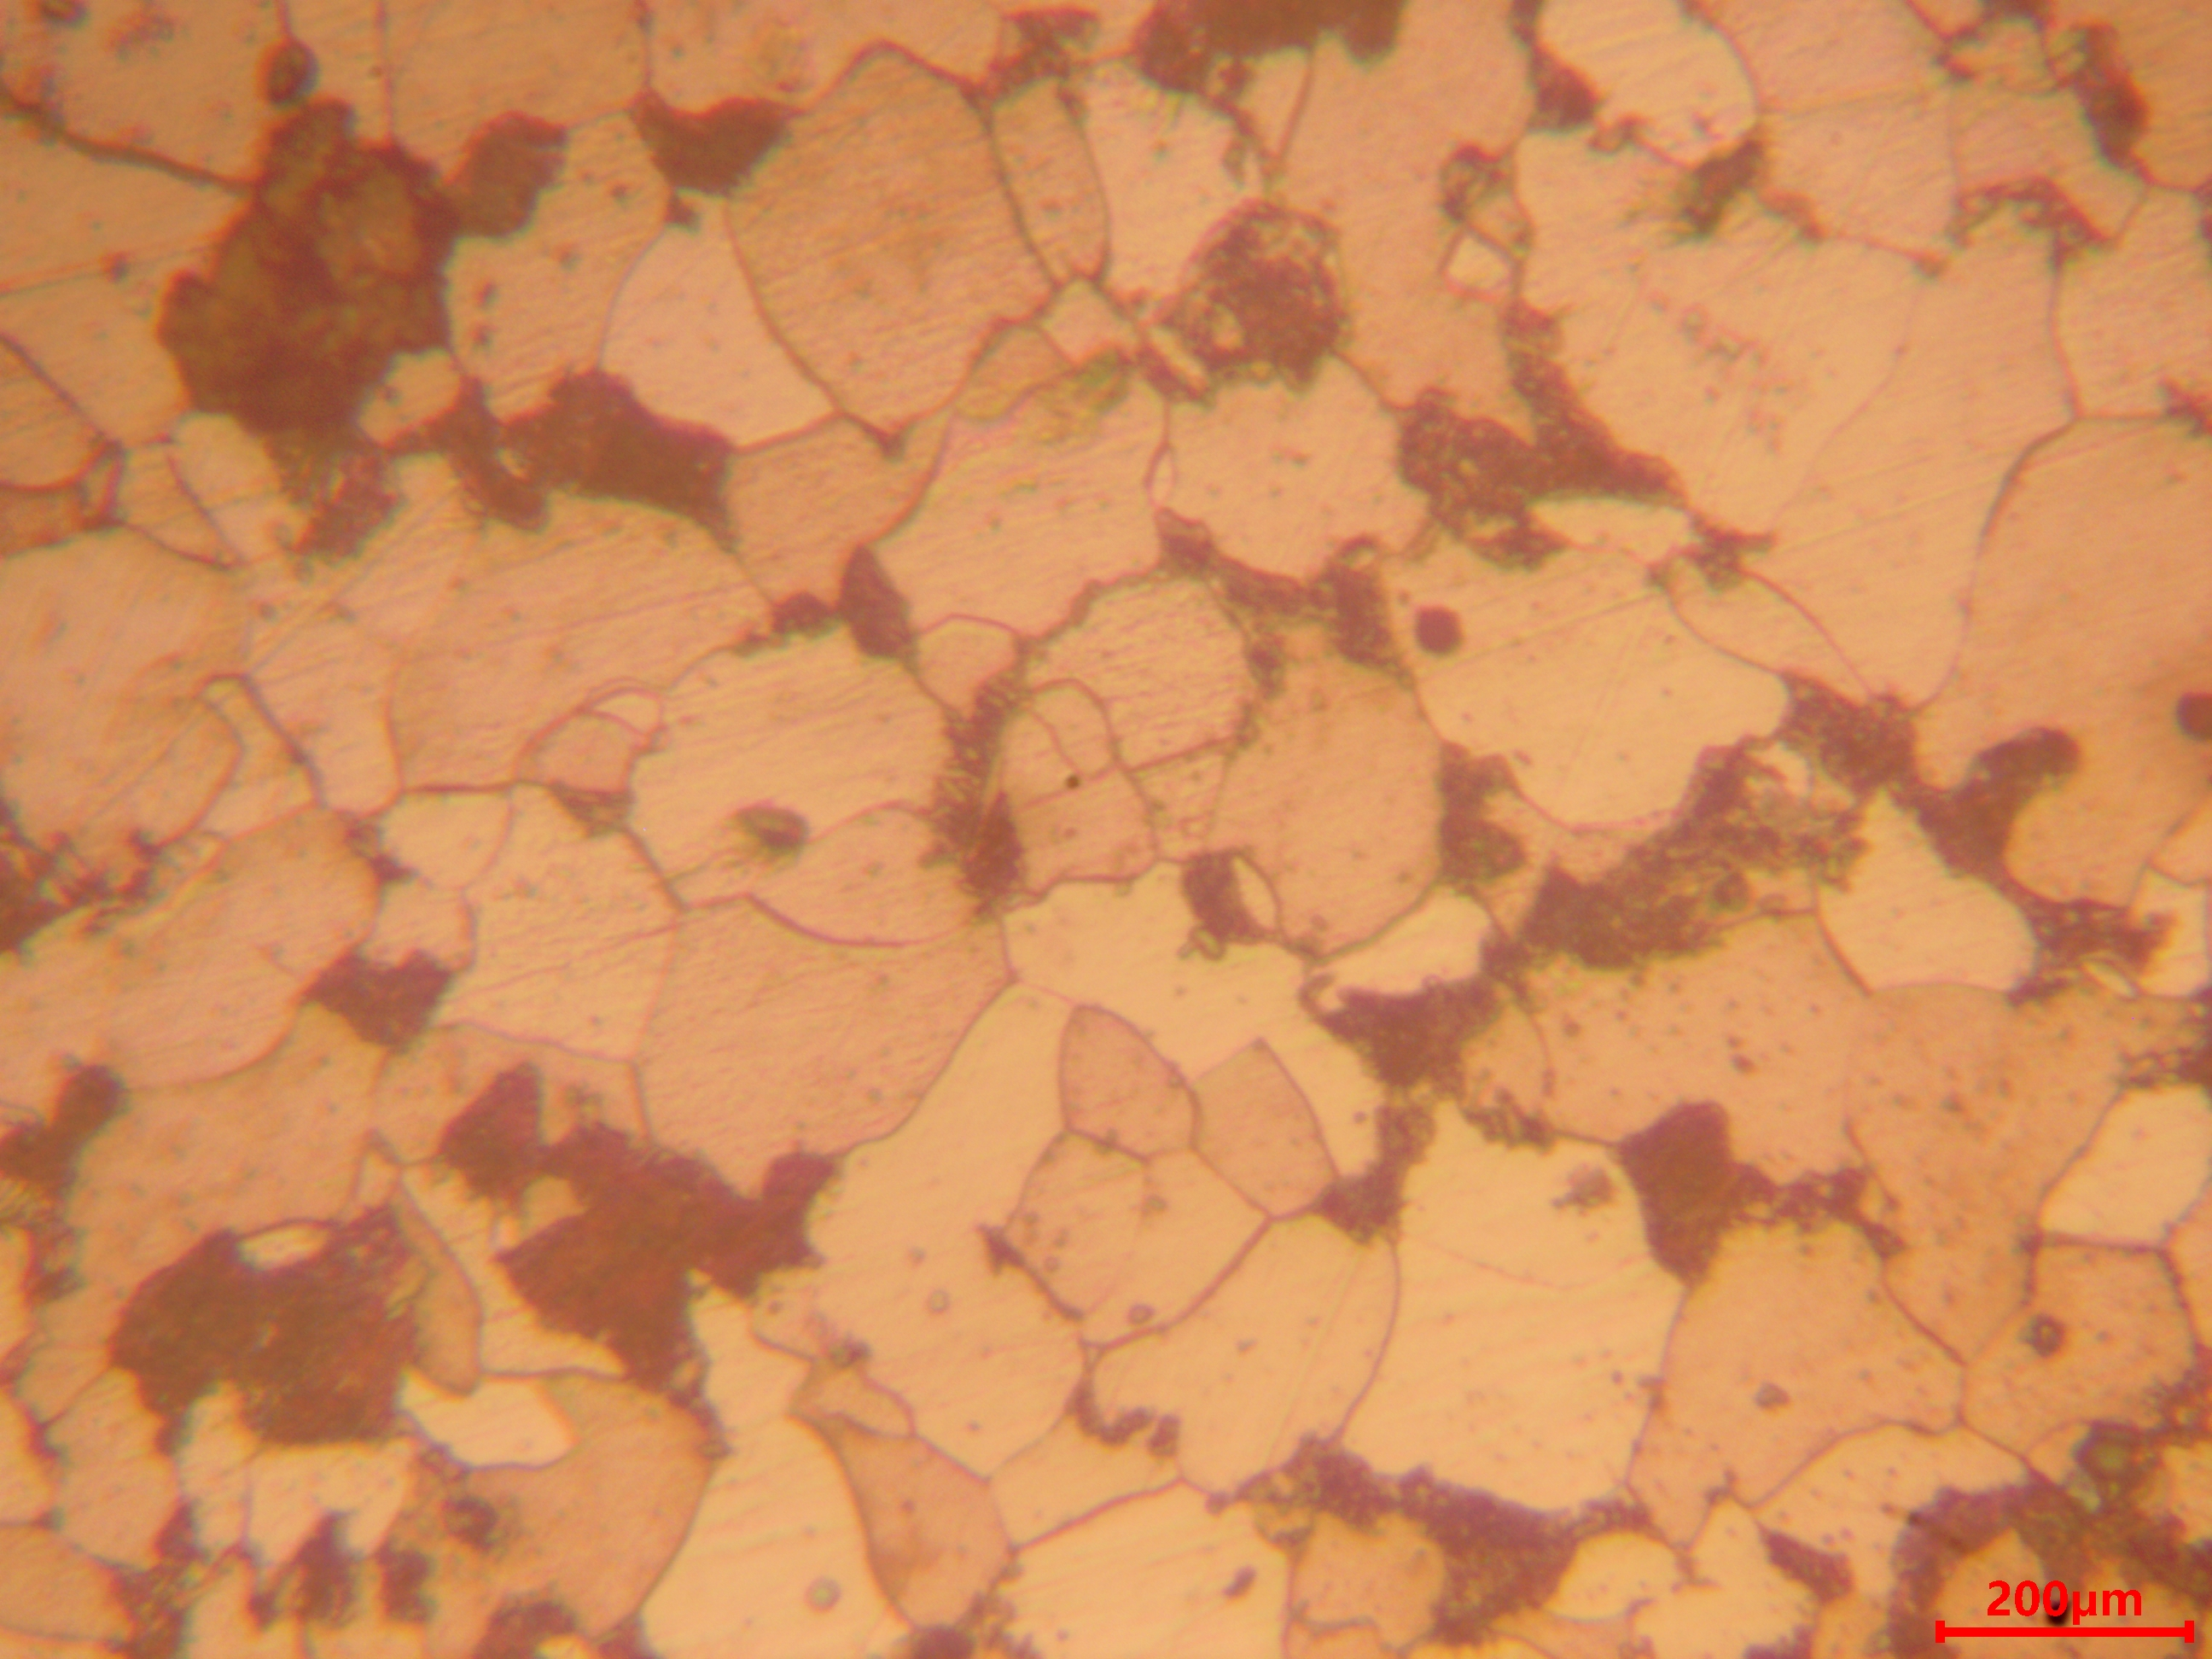
\includegraphics[width=0.40\textwidth]{exp_img/fig1a.jpg}\label{expfig:fig1a}} \hspace{30pt}
            \subfloat[45 钢水淬 500x]{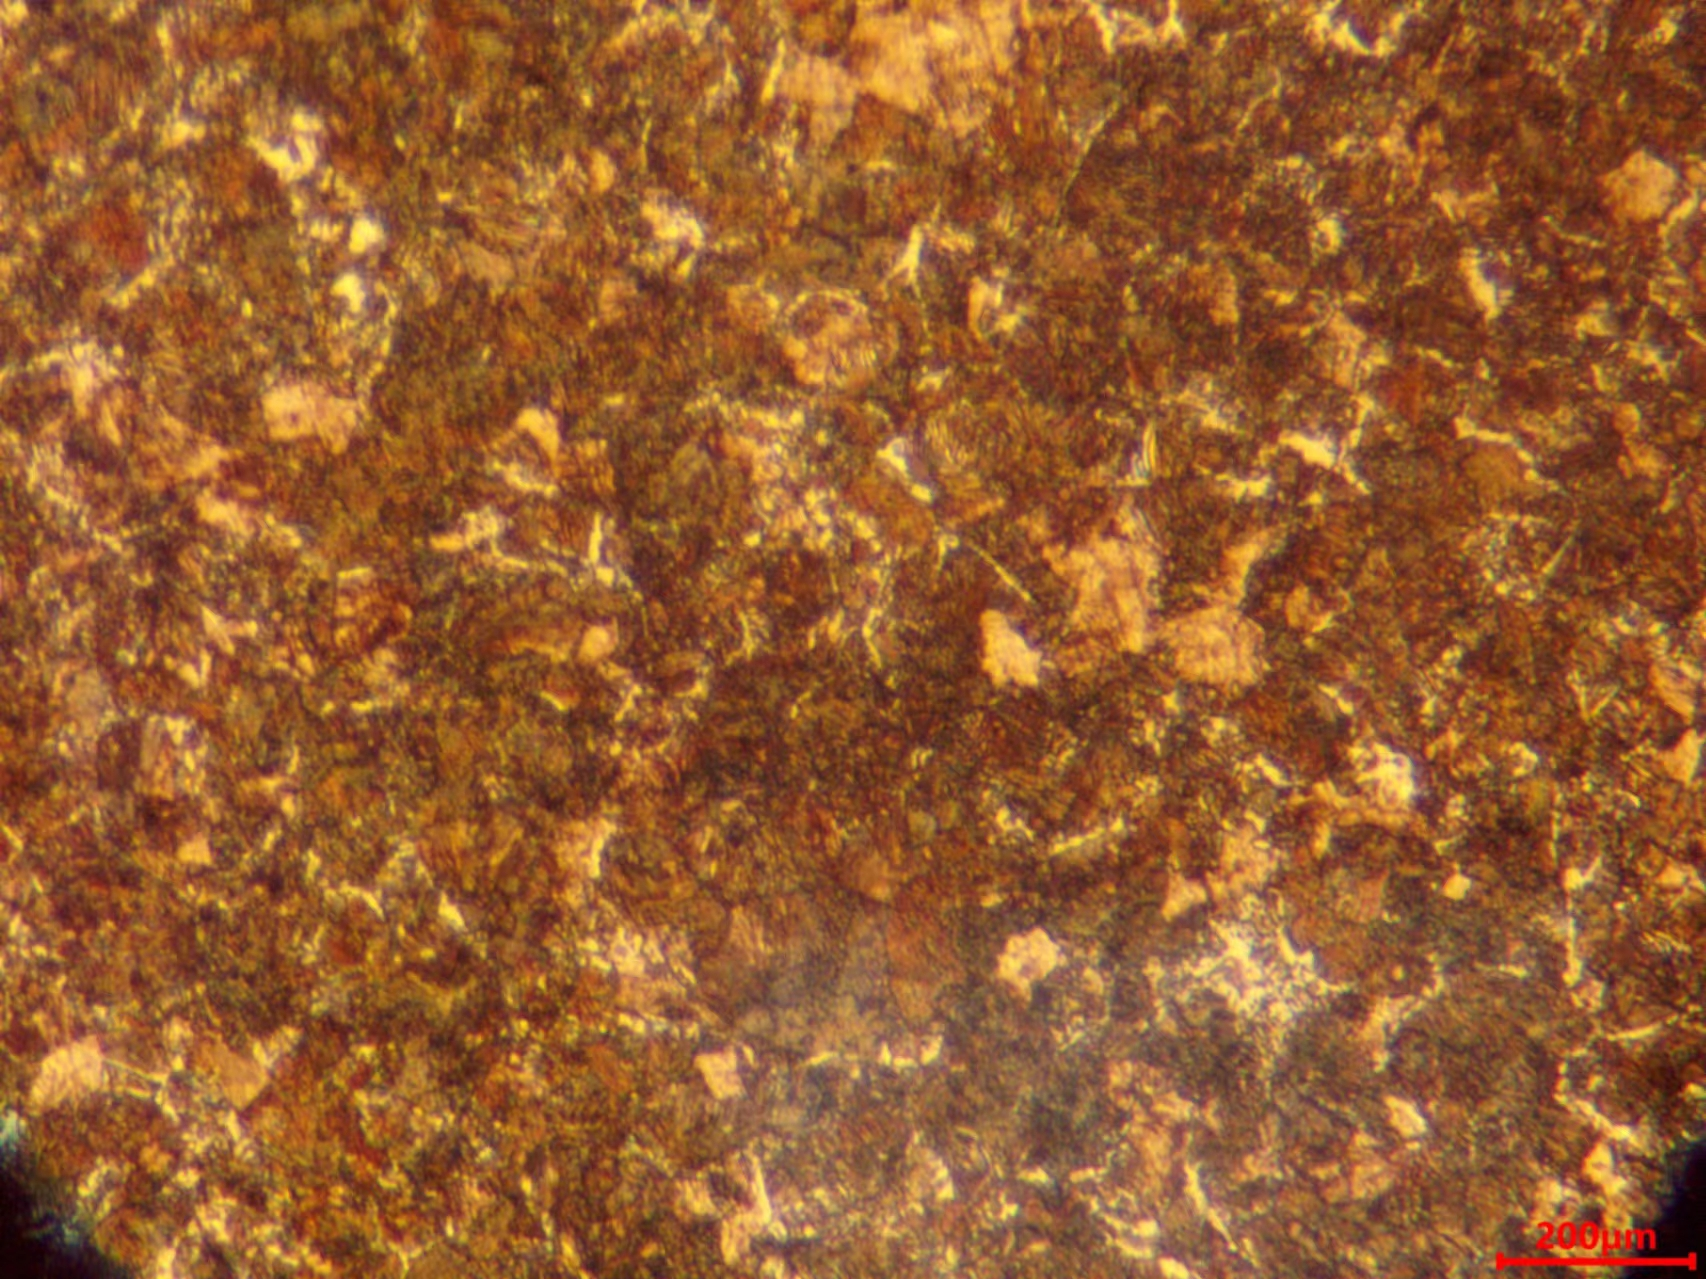
\includegraphics[width=0.40\textwidth]{exp_img/fig1b.jpg}\label{expfig:fig1b}} \\
            \subfloat[45 钢盐淬 500x]{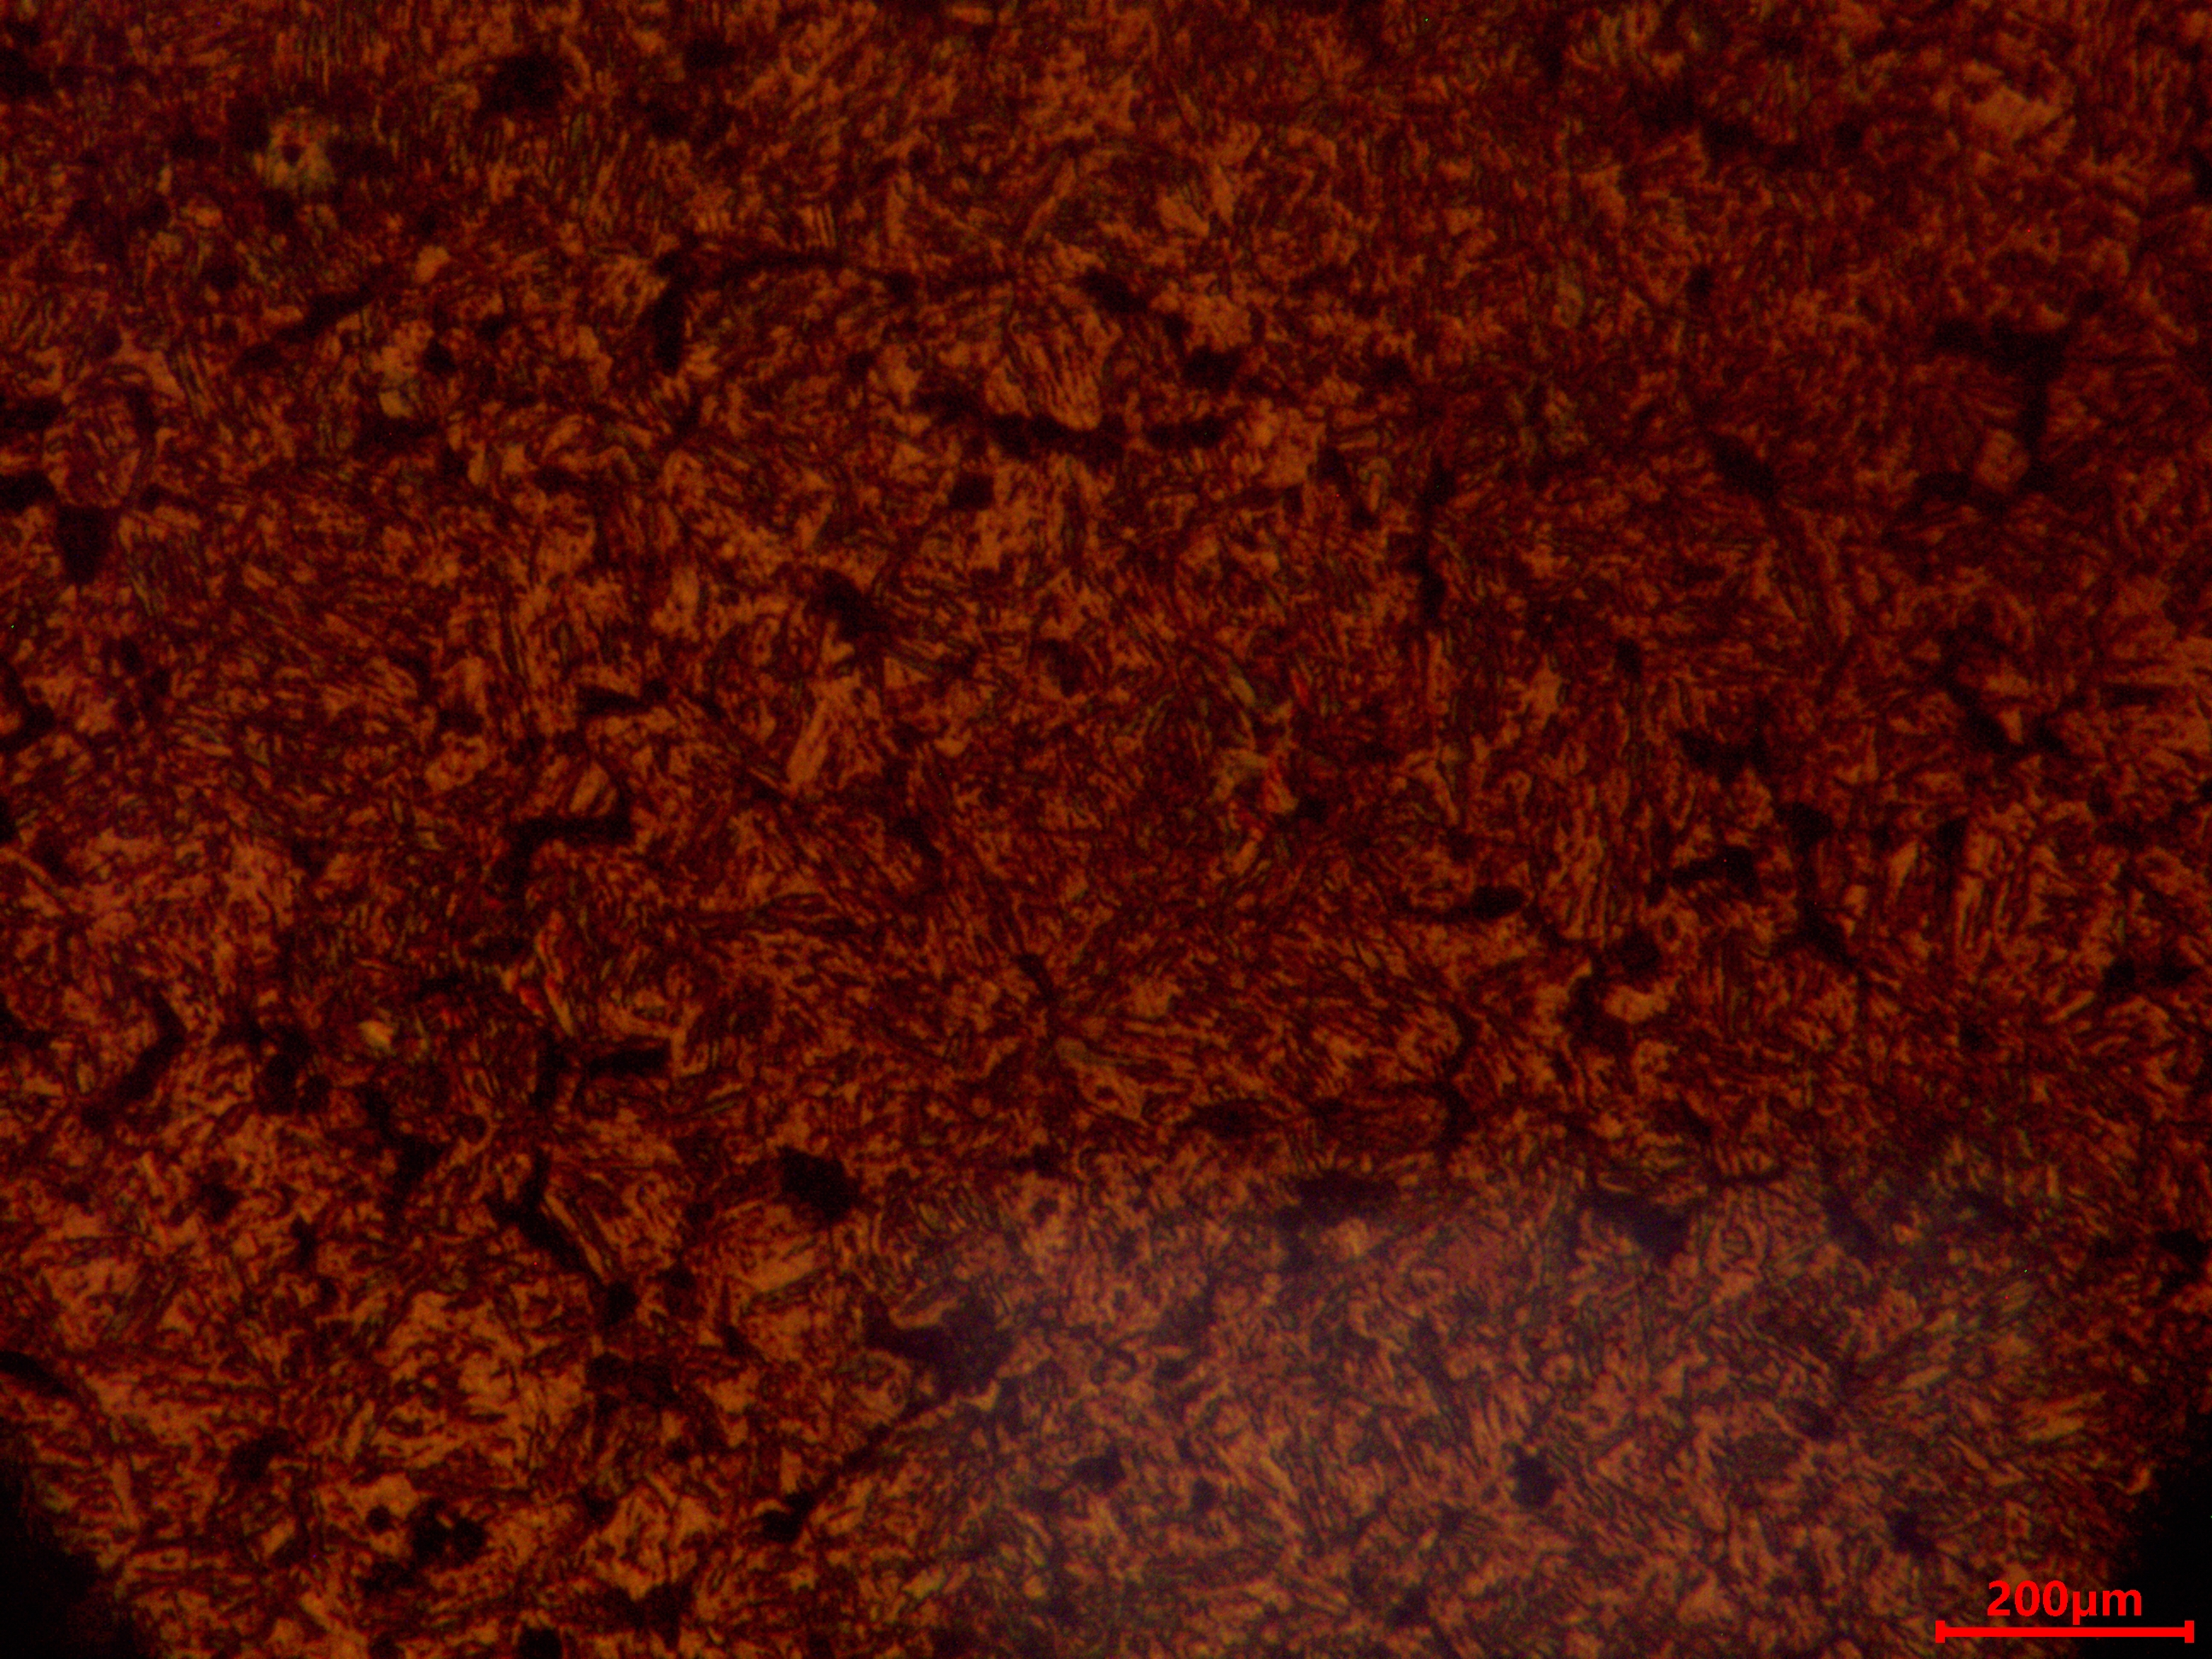
\includegraphics[width=0.40\textwidth]{exp_img/fig1c.jpg}\label{expfig:fig1c}}\hspace{30pt}
            \subfloat[45 钢水淬 低温回火后 500x]{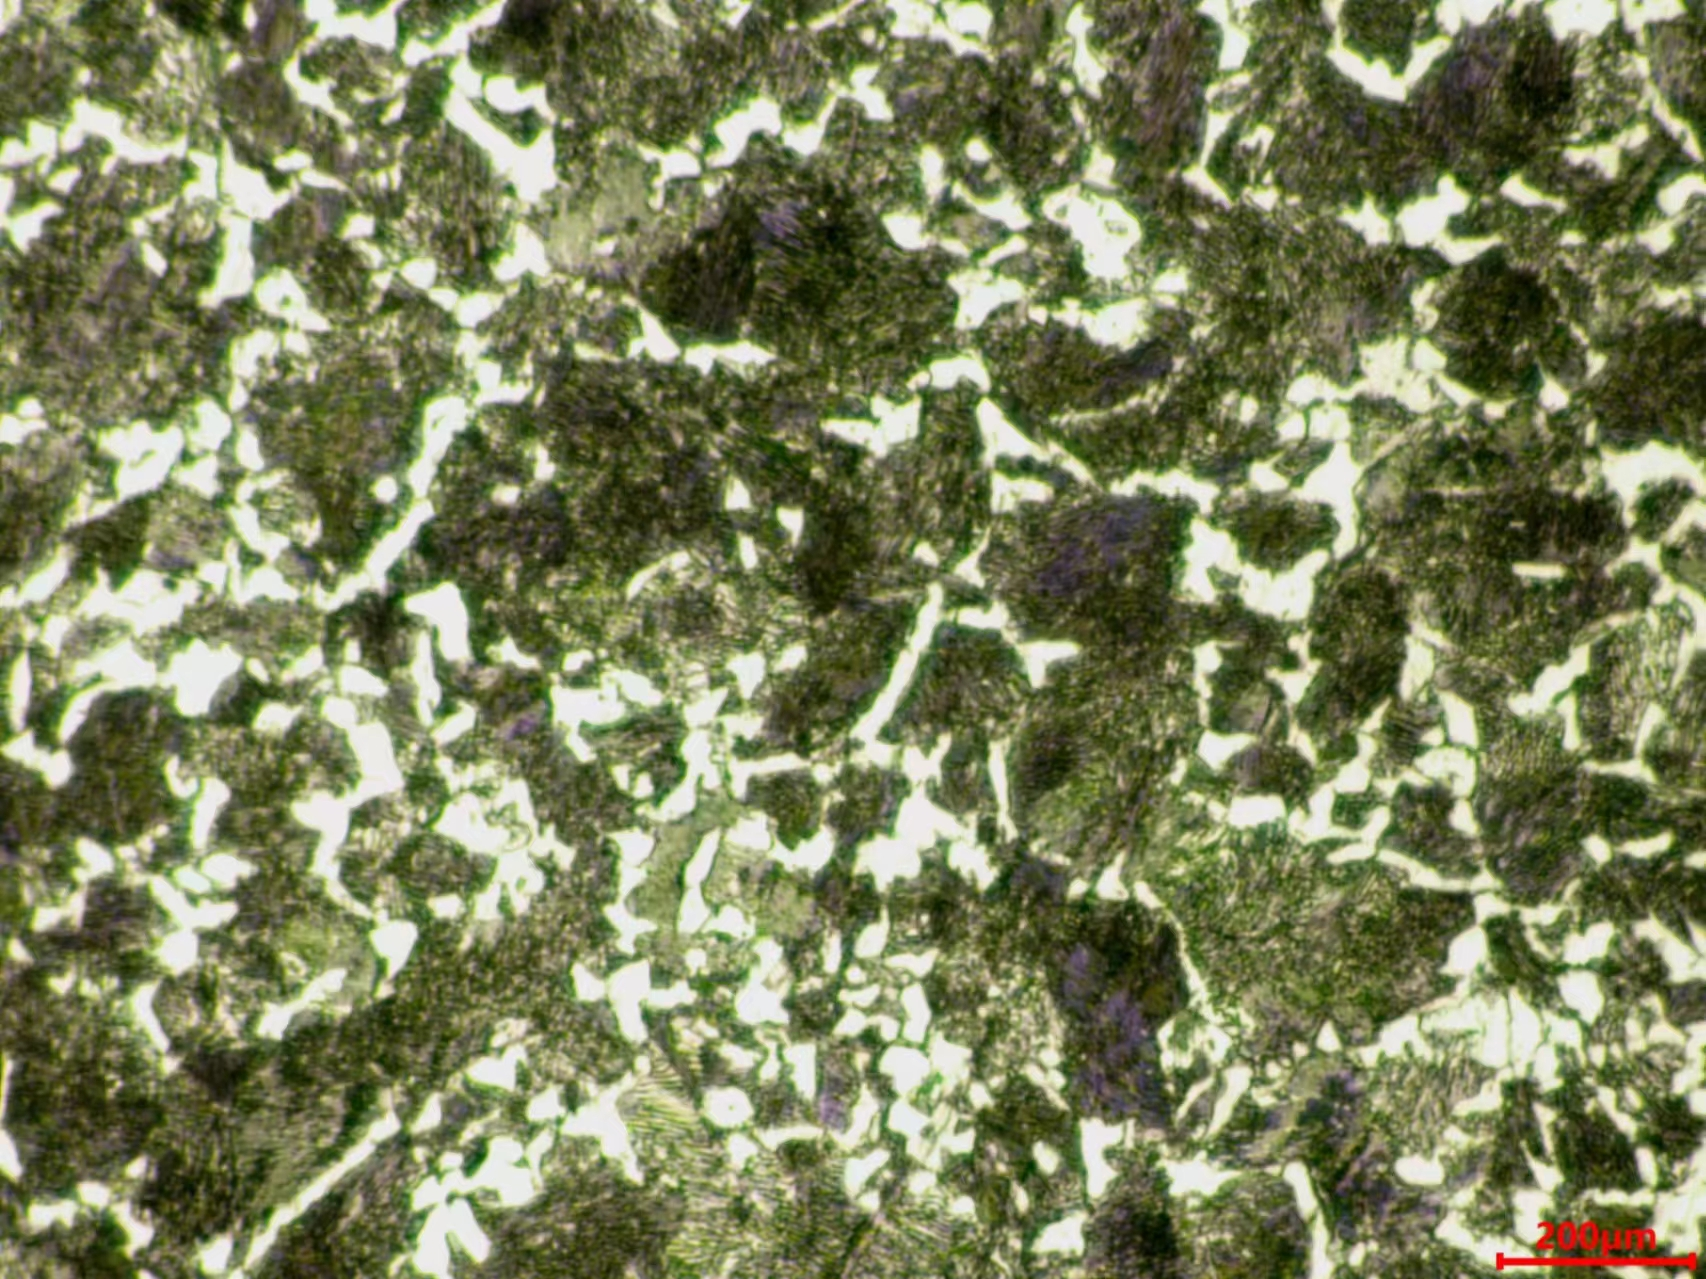
\includegraphics[width=0.40\textwidth]{exp_img/fig1d.jpg}\label{expfig:fig1d}} \\ 
            \subfloat[45 钢水淬 中温回火后 500x]{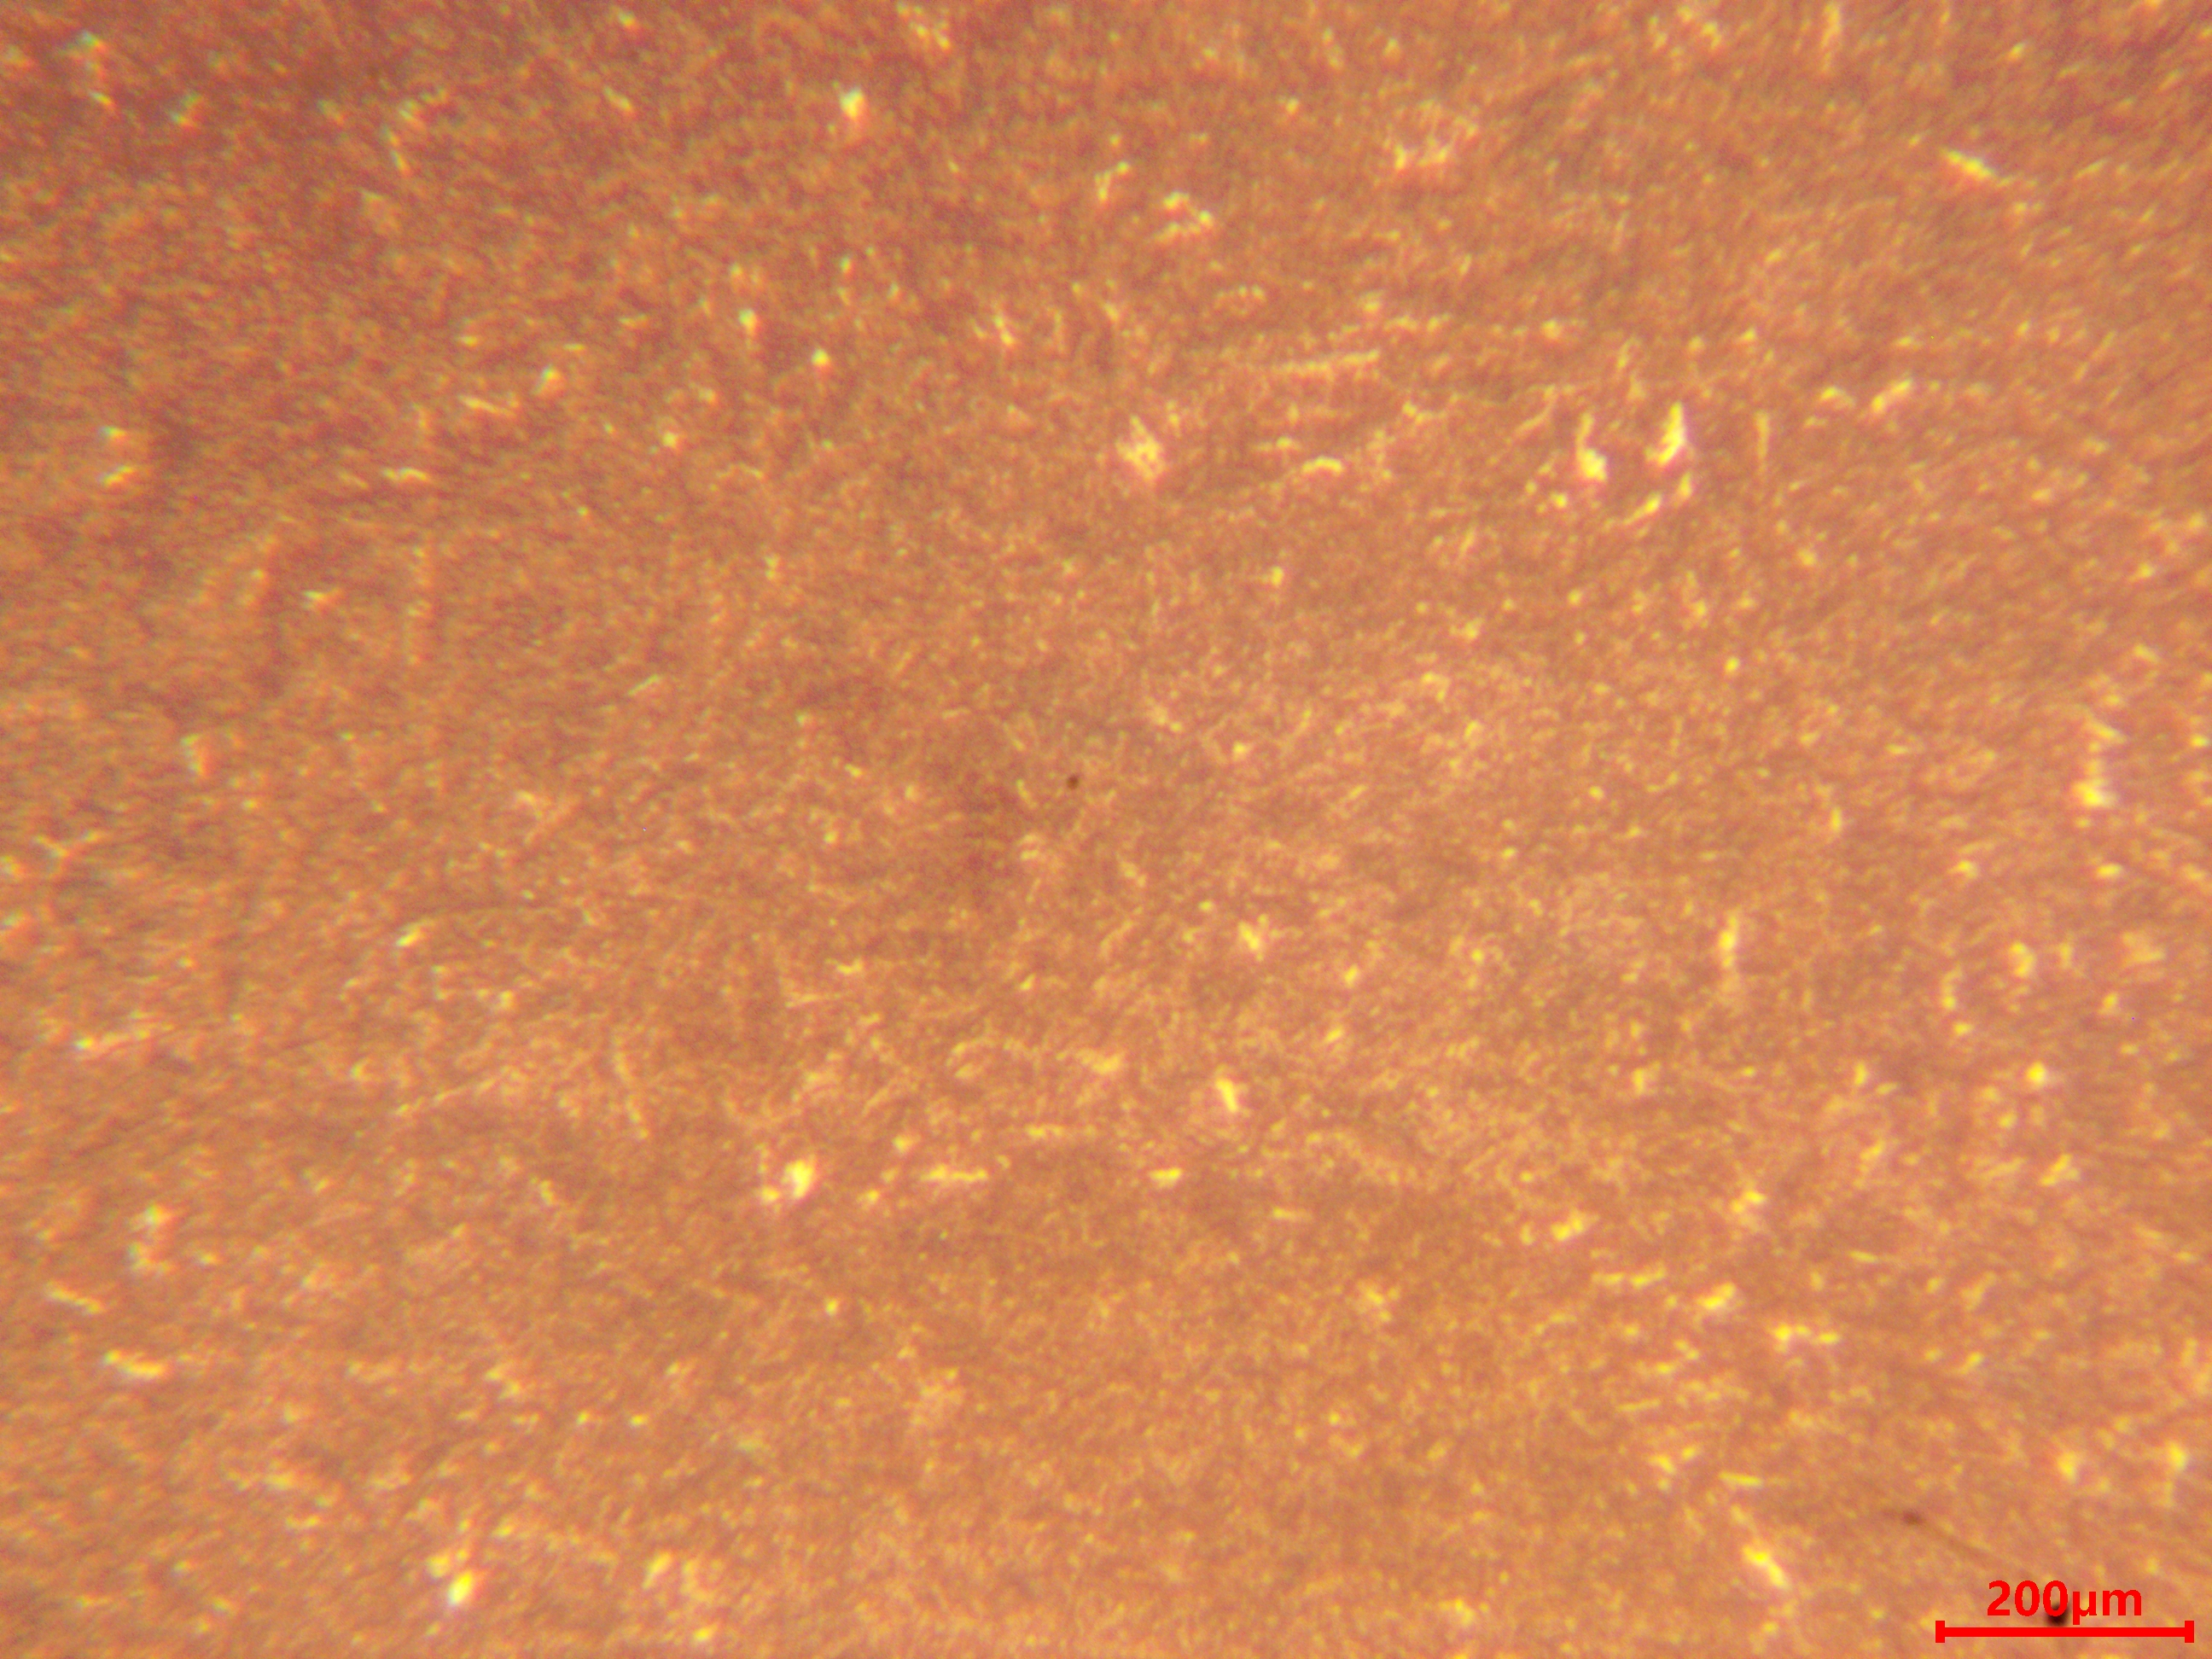
\includegraphics[width=0.40\textwidth]{exp_img/fig1e.jpg}\label{expfig:fig1e}} 
            \hspace{30pt} 
            \subfloat[45 钢水淬 高温回火后 500x]{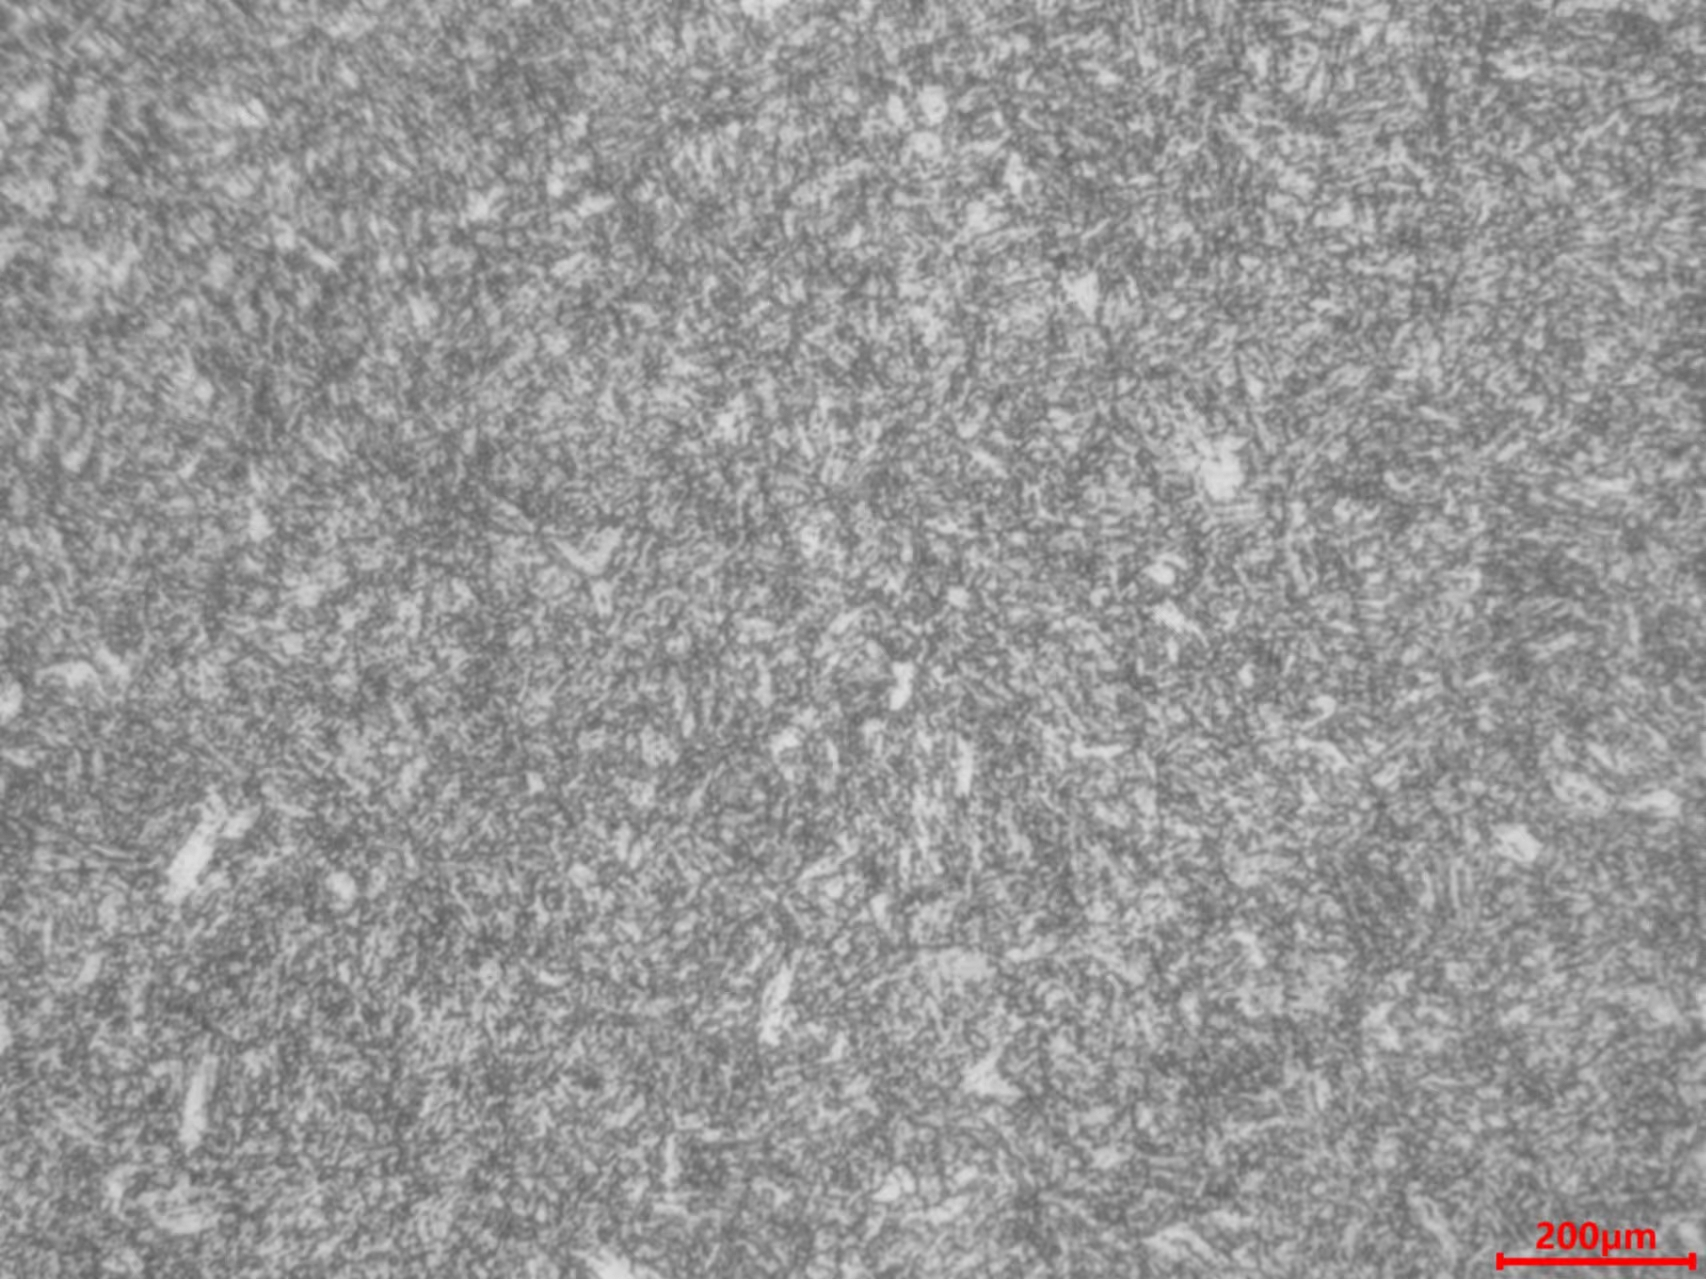
\includegraphics[width=0.40\textwidth]{exp_img/fig1f.jpg}\label{expfig:fig1f}} \\
        \end{figure}
    \subsection{结果分析}
        \subsubsection{淬火工艺}
            三种淬火介质按照冷却速率从大到小依次排序分别为:盐水、水、油。而淬火降温速度越快,则越容易得到较硬的马氏体相,这与得到的三种试样的淬火后硬度完全吻合。再来看金相图,随着介质的冷却速率提升,我们可以明显看出金相组织的粒度急剧缩小,从油淬样品中粗大而均匀的大晶粒最终变成盐淬样品中细小针状的细密晶粒,这些针状或板条状的深色结构正是我们想要得到的马氏体相。\par
            至于为什么主要成分同样是水,盐水淬能比水淬获得更理想的马氏体结构,这要考虑到一个特殊性质:当冷却介质为 20 ℃ 的自来水,工件温度在 200 $\sim$ 300 ℃ 时,平均冷却速度为 450 ℃/s;工件温度在 340 ℃时,平均冷却速度为 775 ℃/s;工件温度在 500 $\sim$ 650 ℃ 时,平均冷却速度为 135 ℃/s。因此,水的冷却特性并不理想,在需要快冷的 500 $\sim$ 650 ℃ 温度范围内,它的冷却速度很小,而在 200 $\sim$ 300 ℃ 需要慢冷时,它的冷却速度反而很大。查阅资料得知:钢加热到奥氏体后,只有冷却速度大于临界冷却速度时才能获得马氏体组织。因此,理想淬火冷却介质的性能是使钢在高温区域( 700 ℃ 以上)较缓慢地冷却,以减少工件的热应力;在 550 $\sim$ 600 ℃ 间以足够快的冷却速度迅速通过奥氏体等温转变图的“鼻尖”,以防止发生珠光体或贝氏体转变;在容易造成淬火裂纹的过冷奥氏体较稳定的低温区域( 300 ℃ 以下)缓慢冷却,使工件在缓冷条件下通过奥氏体向马氏体的转变区,从而减少相变应力。而盐溶液的蒸汽压使其刚好能满足上述要求,故可以得到更理想的马氏体结构。
        \subsubsection{回火工艺}
            如 \fgref{fig2} ,随着回火温度越来越高,回火后的硬度下降幅度越来越大。\par
            \begin{figure}
                \caption{硬度减少量随温度变化曲线\label{fig2}}
                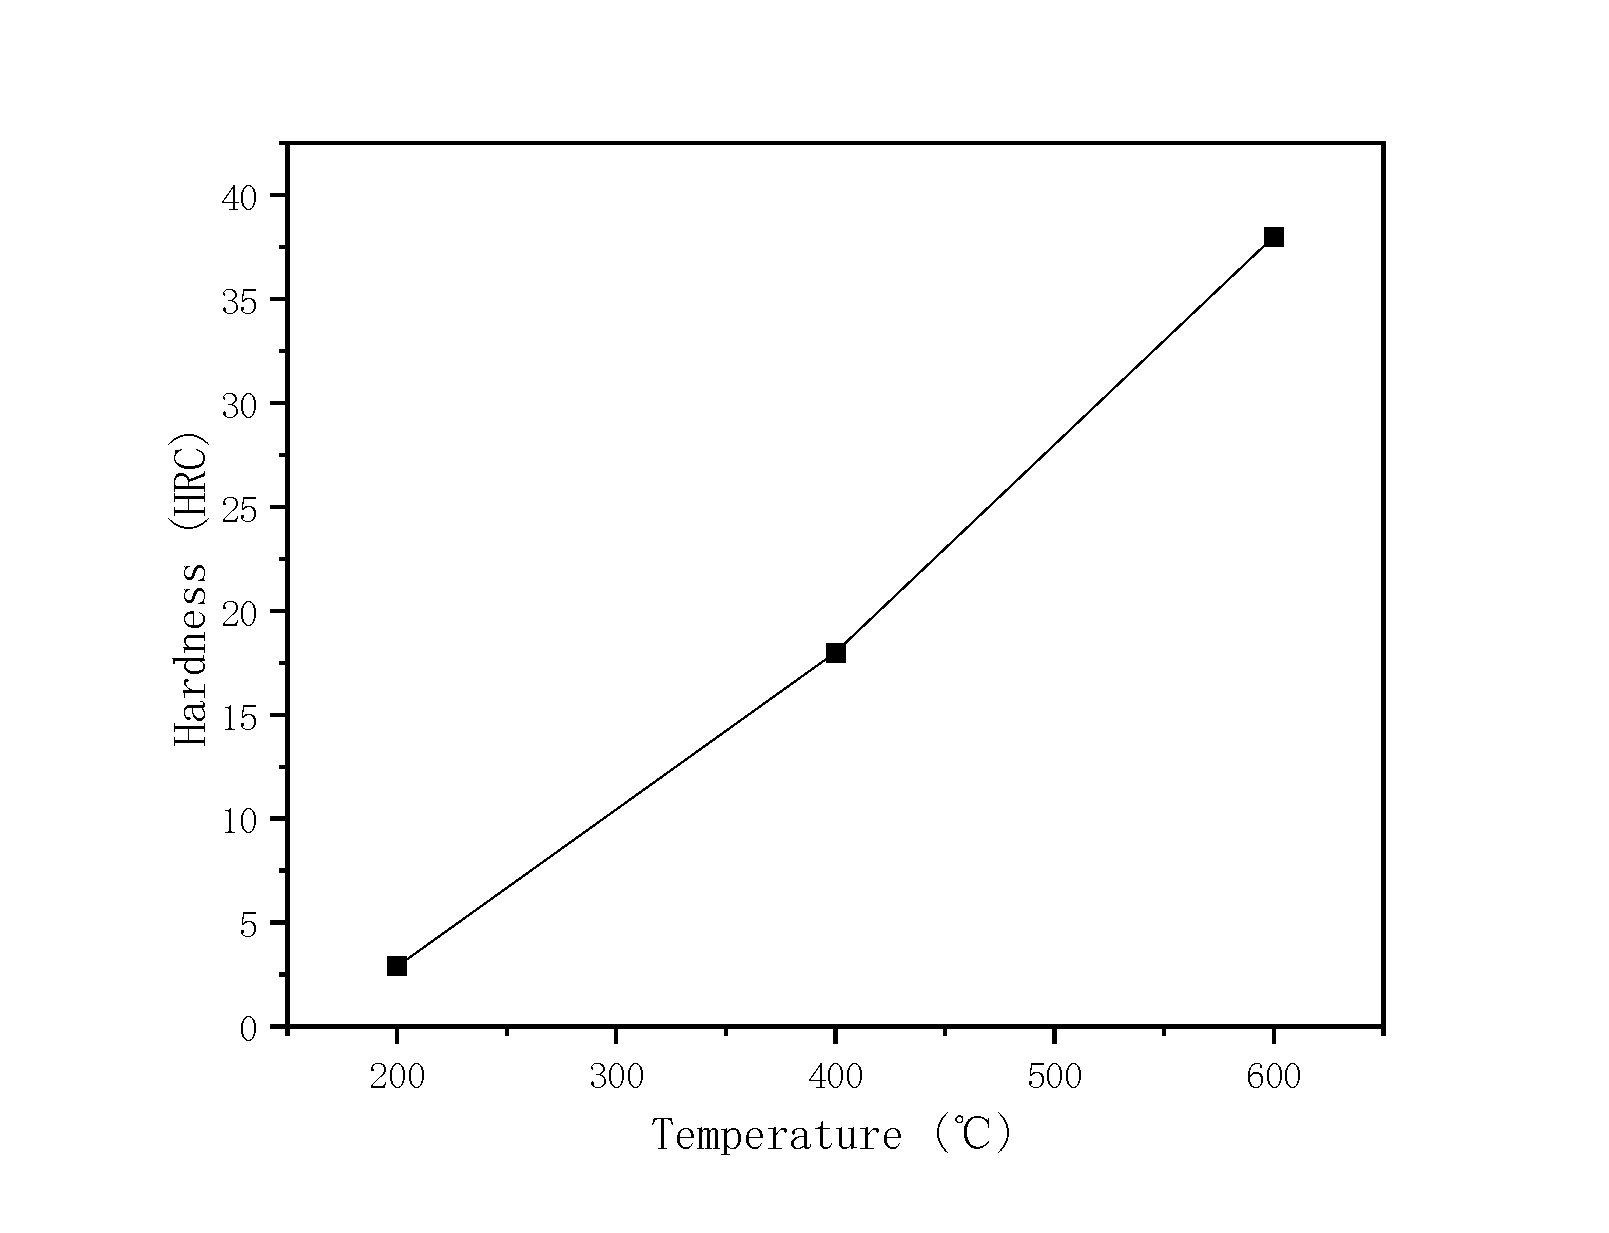
\includegraphics[width=0.5\textwidth]{exp_img/fig2.pdf}
            \end{figure}\par
            一方面回火可以释放内应力,让组织结构更加稳定,韧性提高、但硬度下降。另一方面是随着回火温度的升高,马氏体回火的比例提高,这使得钢材损失一部分硬度、但是可以得到更大的韧性。金相图显示,200℃ 回火时,有部分马氏体分解,形成了细小的回火马氏体组织; 400℃ 回火时,马氏体结构进一步分解转变为细小的回火索氏体,由小尺寸的铁素体和碳化物均匀混合得到;这一现象在 600℃ 回火时非常显著,整个金相结构都转变为了均匀的灰色组织,这正是回火索氏体。
\section{思考题}
    \subsection{45 钢淬火后硬度不足,如何用金相分析来断定是淬火加热温度不足还是冷却速度不够?}
        如果淬火加热温度不足,通常会导致试样中的组织结构未完全转变为马氏体。在金相分析中,观察试样的组织结构是否存在未转变为马氏体的组织相,如珠光体或渗碳体,可以判断加热温度是否达到足够高的临界温度。\par
        如果淬火后的试样中存在未转变为马氏体的组织相,并且淬火后的组织结构呈现出较粗大的珠光体或渗碳体,这可能是由于冷却速度不够快所致。在金相分析中,观察试样的组织结构是否存在较大的珠光体或渗碳体,以及马氏体的比例较低,可以判断冷却速度是否达到足够快的水平。
\end{document}